\documentclass[12pt]{article}
\usepackage[utf8]{inputenc}
\usepackage{graphicx}

\title{Master's thesis proposal}
\author{Cristian Manuel Abrante Dorta}
\date{July 2021}

\begin{document}

\maketitle

\section{Introduction}

During recent years there has been some discussions about how to correctly organize and deploy service oriented architectures. One of the software architecture patterns that has gained more popularity nowadays are microservices. Many big, mid-level and even small software companies had adopted this architecture due to its tremendous benefits in comparison with traditional and monolithical software applications. \\

Microservices are basically an extension of service oriented architecture. The main goal, is that each of those microservices offer a well-defined and clear scope of functionalities, that can be accessed by another microservice using \textit{remote procedure calls} \cite{nelson1981remote}. The main advantage of this pattern is that it can be established a clear ownership of each microservice by different teams where they are responsible for the development, maintenance and deployment of them. This presents a clear advantage in comparison to the classical \textit{monolithic} architecture, because on those, even though the development tasks could be divided in different teams, the deployment of a single functionality implies the deployment of all the system, being then prone to cause important problems that can shut down completely the application. \\

Even though microservices architecture represents an step forward in the design of software systems, it also have some drawbacks in comparison with the monolithic architectures, such as the performance. In traditional monolithic application the calls to subroutines is something that can be resolved inside the same process and machine, however in microservices, the call have to be done over the network, which is something that can eventually introduce some delays in the execution. Apart from this, there is another problem that microservices architectures have to face, which is the handling of over thousands of different microservices, when considering businesses that operates at big scale. In this case, any issue caused by one microservice, can be extended through many of them, and engineers have to debug calls that comes from a huge stack different services which is something that can be challenging and time-consuming.\\

This is why many companies had adopted the pattern of \textbf{Domain-Oriented Microservice Architecture} \cite{DOMAUber}. Using this architecture, many microservices can be grouped inside a logical division that can fit the needs of the company. Those logical divisions are called \textbf{Domains}. For isolate the domains and make easier their maintenance and debugging, one approach that many companies had applied is to create a common gateway that expose the interface (usually as routes that can be called with different HTTP methods). Apart from being the single entry point for specific domains, the gateway can also provide different high-level responsibilities, such as authentication, routing, rate limiting, load ballancing etc. This pattern had been widely adopted by companies that operate at a high level such as Uber \cite{GatewayUber}, or Unity Technologies.\\

\begin{figure}[h]
    \centering
    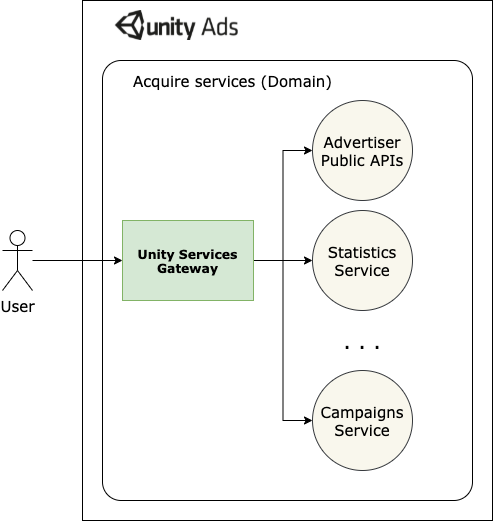
\includegraphics[scale=0.35]{src/proposal/img/unity-services-diagram.png}
    \caption{Unity Acquire microservices architecture setup}
    \label{fig:unity-services-diagram}
\end{figure}

Taking into consideration all this concepts, this thesis aim is to focus on the particular case of the Acquire division of Unity Technologies (Figure \ref{fig:unity-services-diagram}). Unity Technologies is a company based on the United States whose aim is to create tools that help developers to create games and other 3D products. It also runs UnityAds, one of the biggest advertisement networks in the world, and which is one of the main income sources that the company offers to the creators in order to run a successful business out of their games. The Acquire division contains all the tools for the publishers to create and run different advertisement campaigns in their games.\\

From the software perspective, the acquire division can be considered a domain in a Domain-Oriented Microservice Architecture. Functionalities are divided into services that are owned by different teams, and those teams are responsible for their development and deployment. Furthermore, the domain also contains a gateway (Unity services gateway) that is the entry point for all the microservices. Apart from that, it also implements some common top-level functionalities.\\

The gateway is in itself a service too, and monitoring the state of it is a crucial task for guaranteeing the good health of the overall system. In particular, one type of monitoring that is interesting to do is the logging of the errors that are produced at gateway level, such as organization or rate limiting errors. For many teams, which are responsible of services that depends on the gateway, is common to ask these type of questions: \textit{which users or organizations are hitting our rate limits?}, \textit{Which is the amount or the frequency of authentication errors that our system is having?}\\

Considering the current setup of the system, those questions are not trivial to answer. Because when an error happens at gateway level, it usually sends the corresponding answer to the user but it does not register it in a way that can be easily explored and visualized afterwards. Even though the technology stack where usually those microservices are deployed have a lot of logging and visualization functionalities, for example the Google Cloud environment, usually they have some limitations when crossing infomation that can be interesting at visualization level (for example obtaining some data from databases that are not deployed using the same technological stack).\\ 

Taking all this into account, the objective of this thesis is to propose a method on how to correctly monitor and visualize the top-level errors that the gateway of a Domain-Oriented architecture produce, and how to visualize those errors in an effective way for allowing the communication between the involved teams.

\section{Expected outcomes}

Explain the procedure clearly.

\section{Introduction}

Cloud computing is a novel field whose usage had increased dramatically during recent years. For many businesses, including multinational companies and young startups, the possibility of externalizing IT resources to cloud providers, represents an important reduction in their operational costs. This cost reduction represents a major competitive advantage to them because they can use the resources they have available (which in case of startups might be limited) to implement the software or operations that really are part of their value proposition and reducing the infrastructure maintenance costs.\\

One of the big players in the cloud computing sector is Google Cloud. The cloud infrastructure provided by Google offers services that can improve the development process; such as storage space and basic server capabilities, and also elements for advanced deployment and orchestration of web applications and services, such as Google App Engine, which is perfect for deploying \textbf{applications based on microservices}.\\

The microservices pattern had gained popularity during the recent years as it speeds-up the development time by dividing the responsibilities of the different \texttt{services} involved in a system, and therefore reducing the time-to-market. Also, microservices pattern allows to correctly match organizational needs, as the team division can be established depending on the services that they own.\\

There are many multinational companies that uses microservices pattern for the development of their backend services, some examples are Uber, Netflix or Unity. Considering that, most of them had adopted the necessity of creating a single entry point for all their services: an API gateway. Technically speaking, the API Gateway is just another service, whose main functionality is forwarding the queries that are sent from the external user to the corresponding microservice that can return the desired response. Apart from this, the gateway can implement some high-level responsibilities, such as rate limiting, load balancing or header enrichment.\\

\section{Engineering questions}

Monitoring the activity of the gateway is not an easy task, especially in big companies where the number of queries that it receive can be in the order of thousands per minute. Also the monitoring is something that is not only relevant for the gateway development team, but it is something that it is interesting for all the teams whose develop services under its umbrella.\\

Taking into consideration that the premise of this thesis is working with microservices architecture applications deployed in a Google Cloud environment that had adopted an API Gateway as an entry point, the main objective is to determine which would be the optimal way of monitoring the activity of the gateway, taking into account that it receives a very intense traffic and that the results of the monitoring had to be communicated in a visual way using a cross-organization tool. In that sense, creating an effective monitoring system for the application gateway is something that can bring a lot of value for companies that have a microservices application working in high scale.\\

\section{Expected outcomes}

The expected outcome of this project is the creation of an application that can monitor the errors that occurs in the \textbf{Unity Services Gateway}. This gateway is the entry point of all the public and private services that are used on the advertisers side in the Unity Ads Network.\\

\begin{figure}
    \centering
    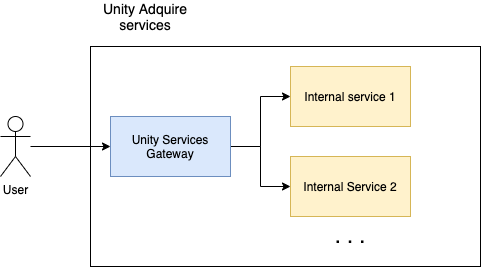
\includegraphics[scale=0.4]{src/proposal/img/diagram-1.png}
    \caption{Current setup of the unity services gateway}
    \label{fig:my_label}
\end{figure}

For the creation of the monitoring application those technologies are going to be used:

\begin{itemize}
    \item \textbf{BigQuery}: Due to the high volume of queries that the gateway handles and the possible amount of errors that can occur in those, it makes sense to use an storage platform that can be scaled to high volumes of data and that can be accessed easily.
    \item \textbf{NodeJS}: The service is written in Javascript and it is using Node.js, so this language and this technology is going to be used for doing the correspondent modifications to it.
    \item \textbf{Grafana}: Grafana is a tool for data visualization and monitoring, it is the standard used in the company so it is going to be used for creating meaningful visualizations for the error events.
\end{itemize}

Taking into consideration the technologies that are going to be used we can create a predefined plan and define the expected outcomes of the project:

\begin{itemize}
    \item Define the structure of the events that are going to be stored in the database. For the proof of concept, the rate limiting error can be used, but this can also be extended to other types of errors in the future.
    \item Add the necessary tables that will contain the events to BigQuery.
    \item Add the functionality of logging the results into BigQuery to the gateway.
    \item Connect Grafana to BigQuery in order to enable error visualization.
\end{itemize}

It is important to remark that this can be considered an iterative process, because as  are developing a software tool, maybe new needs come from different teams or there are some concerns about things that can be improved, so it is important to say that the final result is going to be the result of iterating over the solution.

\bibliographystyle{plain}
\bibliography{proposal}

\end{document}
